\documentclass[../article.tex]{subfiles}

\usepackage[english]{babel}
\usepackage{amsmath}
\usepackage{graphicx}
\usepackage{wrapfig}
\usepackage[superscript,biblabel]{cite}
\DeclareMathOperator*{\E}{\mathbb{E}}
\DeclareMathOperator*{\argmin}{arg\,min}
\DeclareMathOperator*{\argmax}{arg\,max}

\graphicspath{ {./fig/} }

\begin{document}

The main algorithm that I researched for this report was DeepFool, which is an optimized attack method on data for deep neural network classifiers. This technique was first proposed by Moosavi-Dezfooli et al. in their paper, \emph{DeepFool: a simple and accurate method to fool deep neural networks}. The primary attack vector of DeepFool is to introduce instability into a classifier through adversarial perturbations, where minor changes are made to data samples that result in a classifier giving an incorrect output. What distinguishes DeepFool, however, is that it optimizes its attack to have the minimal amount of perturbations applied to the sample data that still tricks a classifier.

\begin{wrapfigure}{r}{0.25\textwidth} %this figure will be at the right
	\centering
	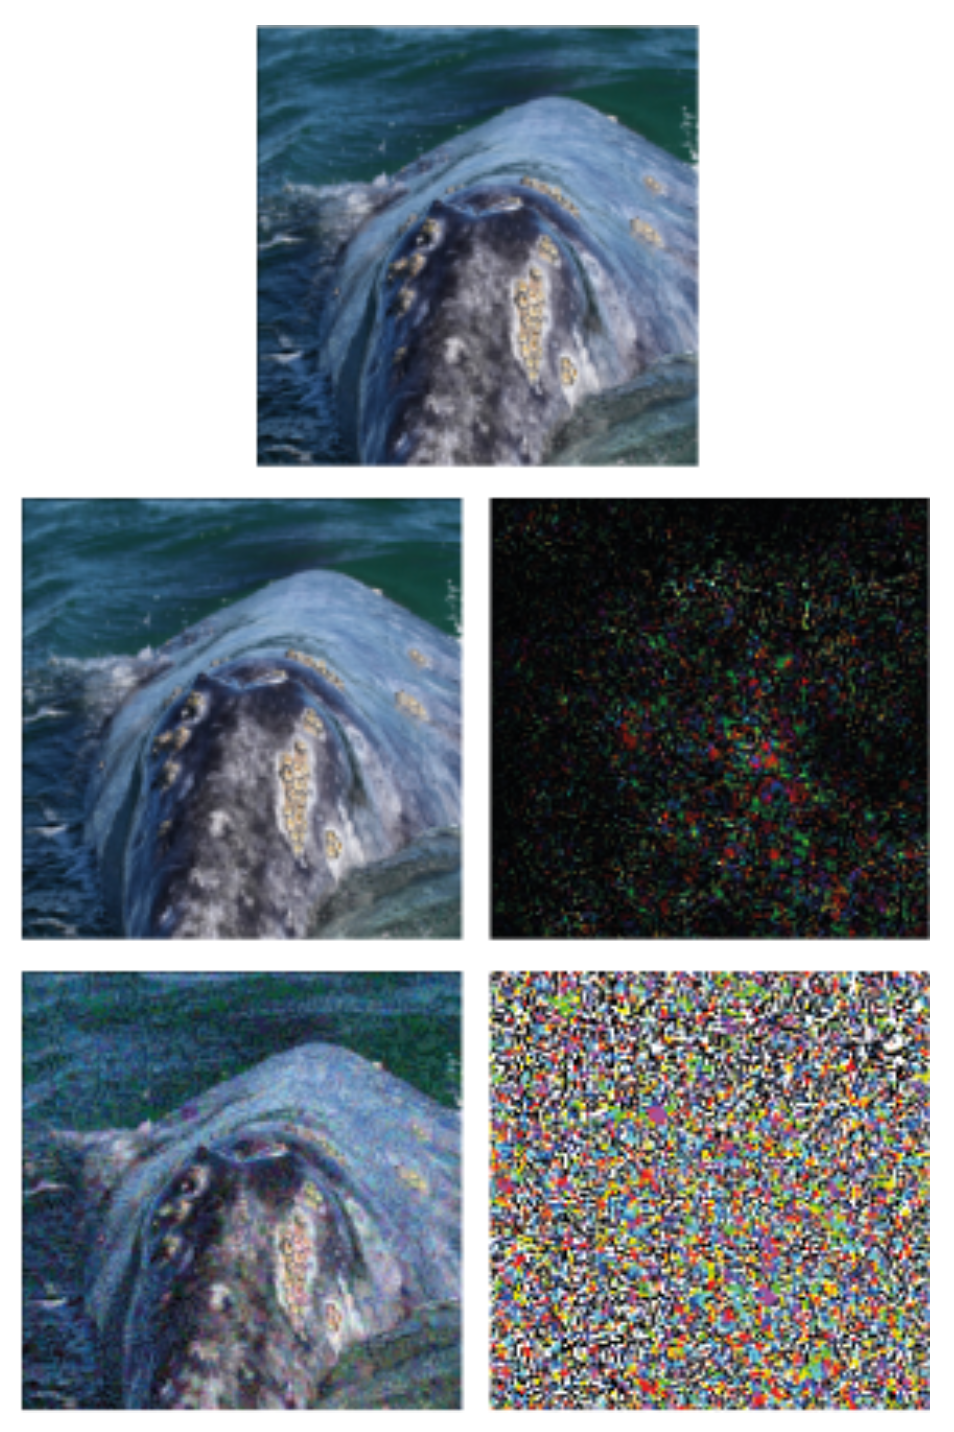
\includegraphics[width=0.25\textwidth]{adv_pert_img.png}
	\caption{\label{fig:Figure 1}Base image (top row). Image perturbed and perturbations by DeepFool (middle row). Image perturbed and perturbations by fast gradient sign method (bottom row).}
\end{wrapfigure}

Adversarial perturbation has seen extensive research outside of DeepFool. First thoroughly explored by Szegedy et al. in 2014, existing research aims to approximate the minimum number of perturbations required to fool a deep neural network classifier. However, their optimization method does not scale to larger datasets. These techniques are often overly-expensive in terms of computation, such as the method Nyugen et al. developed to render a data sample unrecognizable to a human, but convince a classifier to classify it with confidence. Other researchers created a fast gradient step method, which quickly calculate approximately optimal perturbations, but this estimation can be considerably different from a more optimal solution. Figure 1 demonstrates the perturbations created by DeepFool and those created by the previously-mentioned 'fast gradient step' method. The image was originally classified as a whale, and the noise maps in the right column are the perturbations applied to that image in order for the classifier to declare the augmented image as a turtle instead. It can be clearly observed that DeepFool's perturbations are more minimal in quantity and in their affect on the base image, and was able to achieve the same desired misclassification as the gradient step method.

DeepFool's optimized approach to finding the minimal quantity of perturbations stems from the concept of what a perturbation is. First, they defined an adversarial perturbation as the smallest alteration \textit{\textbf{r}} that can change a classifier's estimated label $\hat{k}(x)$ to be the following (ST means "subject to"):

\[\delta(x:\hat{k}) := \min_r||r||_2  ST \hat{k}(x + r) \neq \hat{k}\]

So, let there be some $\hat{k} = sign(f(x))$, where $f(x)$ is an affine, arbitrary, scalar classification function. The robustness of this classifier, or how resistant it is to error, can be expressed as:

\[ \rho_{adversarial} (\hat{k}) = \mathbb{E}_x \frac{\delta(x:\hat{k})}{||x||_2}\]

Here, $\mathbb{E}_x$ represents the expectation over the distribution of all data. With these two expressions, the researchers determined that, as an affine classifier, the distances between points on the classifier's affine hyperplane $w^T x + b = 0$ and its robustness could be determined, and subsequently, so too could the minimum number of perturbations required to cross that threshold. When computed linearly, they derived the expression for that minimum number of permutations as:

\[r_*(x_0) := \argmin ||r||_2 ST sign(f(x_0+r)) \neq sign(f(x_0)) = -\frac{f(x_0)}{||w||_2^2 w}\]

\[\argmin_{r_i} || r_i ||_2 ST f(x_i) + \nabla f(x_i)^T r_i = 0\]

Perturbation $r$ at index $i$ is computed, and then the next $x_{i+1}$ is updated. This continues until the classifier estimator $\hat{k}$ changes, and thus the prediction changes to the intended wrong label.

\begin{wrapfigure}{l}{0.4\textwidth} %this figure will be at the right
	\centering
	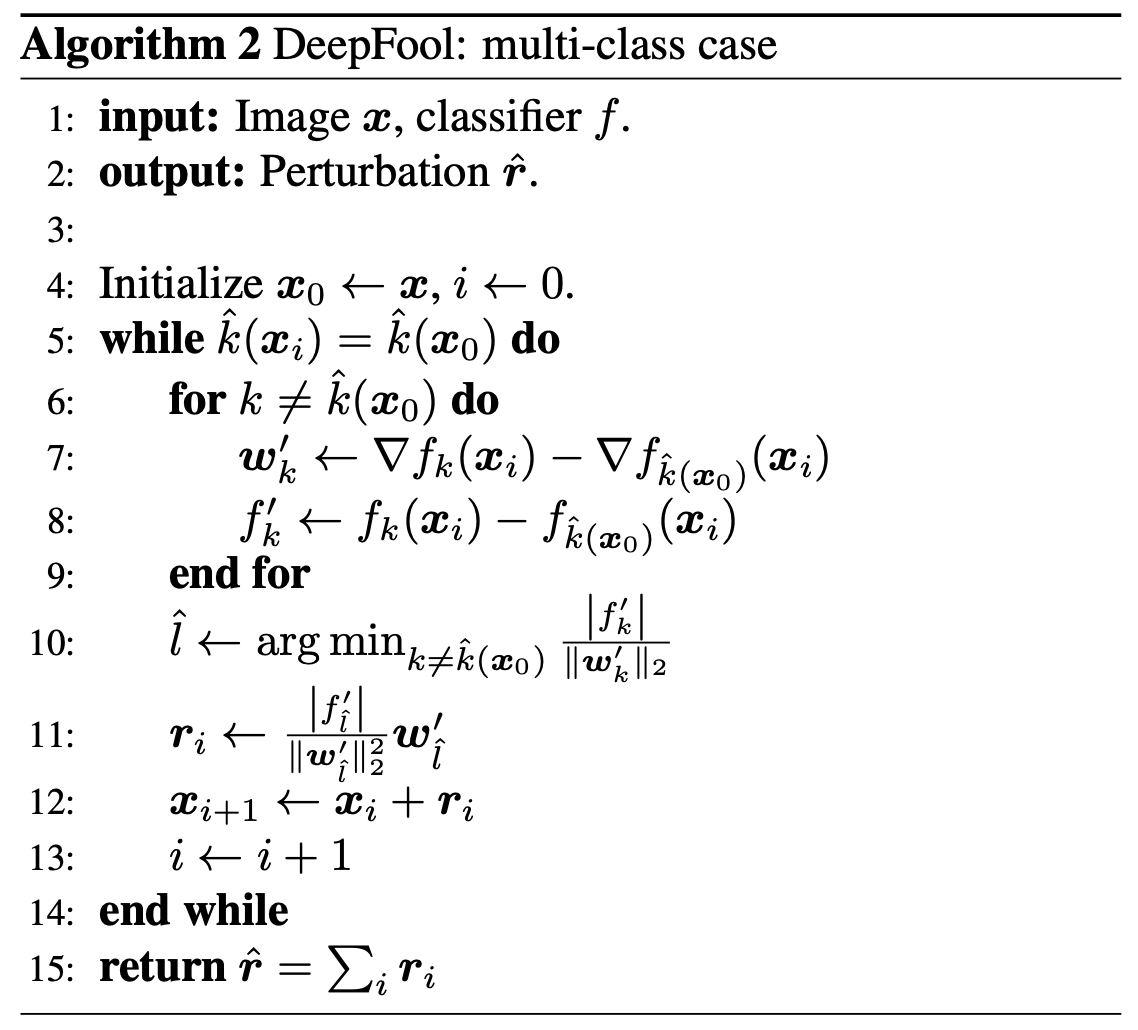
\includegraphics[width=0.4\textwidth]{deepfool_multi_class.png}
	\caption{\label{fig:Figure 2}Pseudocode of the mutliclass iteration of the DeepFool adversarial perturbation attack.}
\end{wrapfigure}

The DeepFool adversarial perturbation optimization method was then expanded to cover mutliclass problem spaces. The researchers treated multi-class classification as an aggregation of binary classification problems, of which the best option is selected. They represent this as, for a classification estimator, $\hat{k}(x) = \argmax_{k} f_k(x)$, where it iterates over each $k$ class. For an affine classifier in this case, an arbitrary classification function can be defined as $f(x) = W^Tx + b$, and the minimum amount of perturbations necessary to change its result is:

\[\argmin_{r} ||r||_2 s.t. \exists k: w_k^T(x_0 + r) + b_k \geq w_{\hat{k}(x_0)}^T (x_0+r) + b_{\hat{k}(x_0)}\] 

This equality is similar in terms of geometric distance to that of the distance between some point, $x_0$, and the complement of a polyhedron $P$ that contains it. In this situation, polyhedron $P$ represents the geometric space equivalent to the classification estimator output $\hat{k}(x_0)$. This problem was solved for with binary classification, however, and that solution can be modified to cover this problem. By letting $\hat{l}(x_0)$ represent the nearest hyperplane to the boundary of polyhedron $P$, the minimum amount of perturbations can then be calculated as a vector that projects the label onto that hyperplane. The final implementation of this derivation can be seen in Figure 2, which depicts the full mutliclass algorithm for DeepFool.

\end{document}